\chapter{NCC}
Please tell more about conclusion and how to the next work of this study.

\section{Lusia Violita Aprilian-1184080}
\subsection{Teori}
\begin{enumerate}
\item Menjelaskan kenapa file teks harus dilakukan tokenizer
	\par Tokenizer adalah untuk membuat vektor dari teks. Dan mengapa harus dilakukan tokenizer? itu karena dengan memfungsikan tokenizer, teks dapat divektorkan. Sehingga teks yang telah telah divektorkan tersebut dapat terbaca pada Machine Learning.
	\par Berikut adalah ilustrasi pemakaian pada tokenizer, perhatikan gambar \ref{7A1}:
		\begin{figure}[!hbtp]
		\centering
		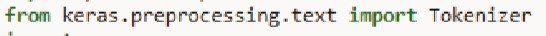
\includegraphics[scale=0.4]{figures/v1.jpg}
		\caption{Lusia-Tokenizer}
		\label{7A1}
		\end{figure}

\item Menjelaskan konsep dasar K-Fold Cross Validation
\item Menjelaskan kode program for train, test in splits.
\item Menjelaskan maksud kode program
\item Menjelaskan maksud fungsi
\item Menjelaskan maksud fungsi
\item Menjelaskan maksud fungsi
\item Menjelaskan maksud fungsi

\item Menjelaskan apa itu Deep Learning
	\par Deep Learning merupakan cabang dari Machine Learning atau bagian keluarga yang lebih luas dari method machine learning berdasarkan pada representasi data pembelajaran. Deep Learning menggunakan Deep Neural Network dalam menyelesaikan suatu masalah yang terjadi pada Machine Learning.

\item Menjelaskan apa itu Deep Neural dan bedanya dengan Deep Learning
	\par Deep Neural Network atau DNN merupakan algoritma yang berbasis neural network yang digunakan untuk mengambil keputusan.
	\par Yang membedakan Deep Learning dengan  Deep Neural Network (DNN) adalah DNN merupakan algoritma yang digunakan pada Deep Learning, sedangkan Deep Learning merupakan model yang menggunakan algoritma DNN.

\item Menjelaskan perhitungan algoritma konvolusi
\end{enumerate}



\par
\par
\par
\par
\section{Fadila-1164072}
\subsection{Teori}
Penjelasan Tugas Harian 12 ( No 1-11 ).
\begin{enumerate}
\item Mengapa File Teks Harus Dilakukan Tokenizer Besera Ilustrasi Gambar :
\begin{itemize}
\item Tokenizer :
\par Difungsikan untuk membuat vektor dari text. Lebih detailnya, tokenizer merupakan langkah pertama yang diperlukan dalam banyak tugas pemrosesan bahasa alami, seperti penghitungan kata, penguraian, pemeriksaan ejaan, pembuatan corpus, dan analisis statistik teks.
\par
\par
\item Mengapa Text Harus Dilakukan Tokenizer ? :
\par Text harus dilakukan tokenizer agar dapat dirubah menjadi vektor. Dari perubahan ke vektor tersebut maka data/textnya dapat dibaca oleh komputer (terkomputerisasi).
\par
\par
\item Ilustrasi Gambar : \ref{chapter-7-tokenizer-fadila}
\par
\begin{figure}[!hbtp]
\centering
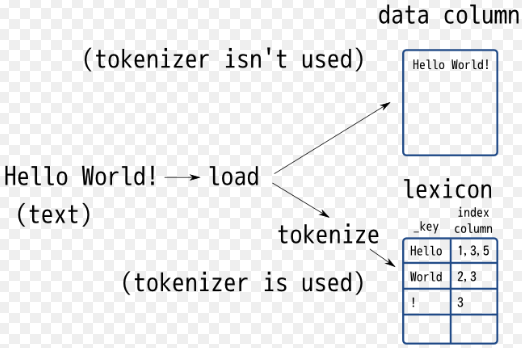
\includegraphics[scale=0.2]{figures/chapter-7-tokenizer-fadila.png}
\caption{Tokenizer - fadila}
\label{chapter-7-tokenizer-fadila}
\end{figure}
\par
\end{itemize}
\par
\par
\item Konsep Dasar K Fold Cross Validation Pada Dataset Komentar Youtube Pada Kode Listing Beserta Dengan Ilustrasi Gambar :
\item Jelaskan Apa Maksud Kode Program For Train Dan Test In Splits Dilengkapi Dengan Ilustrasi Gambar :
\item Apa Maksud Kode Program train\_content = d['CONTENT'].iloc[train\_idx] dan test\_content = d['CONTENT'].iloc[test\_idx] Dilengkapi Dengan Ilustrasi Gambar :
\item Apa Maksud Dari Fungsi Tokenizer = Tokenizer(num words=2000) Dan Tokenizer.fit on texts(train content), Dilengkapi Dengan Ilustrasi Gambar :
\item Apa Maksud Dari Fungsi d train inputs = tokenizer.texts to matrix(train content, mode=’tfidf ’) dan d test inputs = tokenizer.texts to matrix(test content, mode=’tfidf ’), Dilengkapi Dengan Ilustrasi Kode Dan Atau Gambar :
\item Apa Maksud Dari Fungsi d train inputs = d train inputs/np.amax(np.absolute(d\_train) :
\item Apa Maksud Dari Fungsi Di Listing ?? Dengan Parameter Tersebut. [caption=Compile model,label=lst:7.2] model.compile(loss=’categoricalcrossentropy0, optimizer =0 adamax0, metrics = [0accuracy0]) :
\par
\item Apa itu Deep Learning :
\begin{itemize}
\item Penjelasan :
\par Deep learning merupakan sub bidang pembelajaran mesin yang berkaitan dengan algoritma yang terinspirasi oleh struktur dan fungsi otak yang disebut jaringan saraf tiruan.
\par
\par
\par
\end{itemize}
\item Apa itu Deep Neural Network Dan Apa Bedanya Dengan Deep Learning :
\begin{itemize}
\item Penjelasan Deep Neural Network : 
\par Deep neural network adalah jaringan syaraf dengan tingkat kompleksitas tertentu, jaringan syaraf dengan lebih dari dua lapisan. Deep neural netwok menggunakan pemodelan matematika yang canggih untuk memproses data dengan cara yang kompleks.
\par
\item Perbedaan Deep Neural Network Dan Deep Learning :
\par Perbedaan antara deep neural network dan deep learning terletak pada kedalaman model. deep learning adalah frasa yang digunakan untuk jaringan saraf yang kompleks. Kompleksitas ini disebabkan oleh pola yang rumit tentang bagaimana informasi dapat mengalir di seluruh model. Arsitekturnya menjadi lebih kompleks tetapi konsep deep learning masih sama. Meskipun sekarang ada peningkatan jumlah layer dan node tersembunyi yang terintegrasi untuk memperkirakan output.
\par Untuk pemahaman yang lebih baik, diberikan sebuah contoh terkait dengan penjelasan perbedaan antara deep neural network dan deep learning.
\par
\par
\item Ilustrasi Gambar : \ref{chapter-7-beda-deep-neu-dan-deep-learn-fadila}
\par
\par
\begin{figure}[!hbtp]
\centering
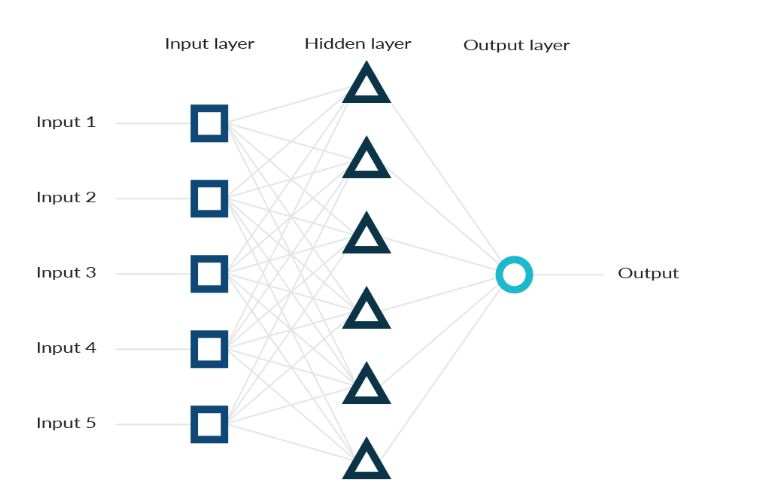
\includegraphics[scale=0.2]{figures/chapter-7-beda-deep-neu-dan-deep-learn-fadila.jpg}
\caption{Perbedaan Deep NW Dan Deep Learn- fadila}
\label{chapter-7-beda-deep-neu-dan-deep-learn-fadila}
\end{figure}
\par
\par
\end{itemize}
\par
\par
\item Bagaimana Perhitungan Algoritma Dengan Ukuran Stride (NPM mod3+1)x(NPM mod3+1) Yang  Terdapat Pada Max Pooling :
\begin{itemize}
\item Penjelasan :
\par
\par
\end{itemize}
\end{enumerate}

\section{Rahmi Roza-1164085}
\subsection{Teori}
\begin{enumerate}
\item Kenapa File Suara Harus Dilakukan Tokenizer
\begin{itemize}
\item Penjelasan: Untuk membedakan karakter-karakter tertentu dalam suatu teks dan juga sebagai pemisah kata atau bukan.Tokenizer dilakukan dengan cara melakukan pemotongan string input berdasarkan tiap kata yang menyusunnya.
\par 
\par
\item Ilustrasi Gambar
\item Tokenizer \ref{teori1}
\begin{figure}[!hbtp]
\centering
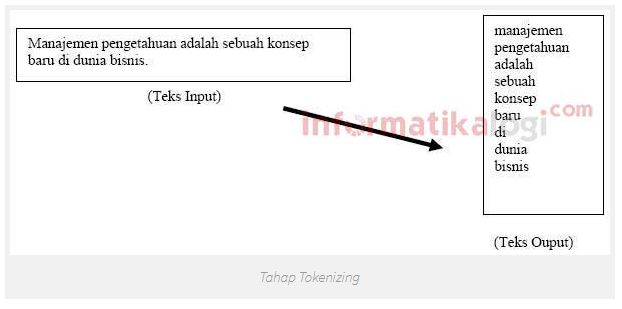
\includegraphics[scale=0.7]{figures/teori1.jpg}
\caption{Tokenizer Roza}
\label{teori1}
\end{figure}
\par
\end{itemize}
\par
\par

\item 	Apa Itu Deep Learning
\begin{itemize}
\item Penjelasan: 
\par  Deep learning merupakan sub bidang pembelajaran mesin yang berkaitan dengan algoritma.
\end{itemize}
\par
\par

\item Apa itu Deep Neural Network Dan Apa Bedanya Dengan Deep Learning :
\begin{itemize}
\item Penjelasan Deep Neural Network : 
\par  Deep neural network adalah jaringan syaraf dengan tingkat kompleksitas tertentu, jaringan syaraf dengan lebih dari dua lapisan.
\par
\item Perbedaan Deep Neural Network Dan Deep Learning :
\par Perbedaan antara deep neural network dan deep learning terletak pada kedalaman model. deep learning adalah frasa yang digunakan untuk jaringan saraf yang kompleks. Kompleksitas ini disebabkan oleh pola yang rumit tentang bagaimana informasi dapat mengalir di seluruh model.
\end{itemize}
\par
\par

\end{enumerate}